\let\negmedspace\undefined
\let\negthickspace\undefined
\documentclass[journal]{IEEEtran}
\usepackage[a5paper, margin=10mm, onecolumn]{geometry}
%\usepackage{lmodern} % Ensure lmodern is loaded for pdflatex
\usepackage{tfrupee} % Include tfrupee package

\setlength{\headheight}{1cm} % Set the height of the header box
\setlength{\headsep}{0mm}     % Set the distance between the header box and the top of the text

\usepackage{gvv-book}
\usepackage{gvv}
\usepackage{cite}
\usepackage{amsmath,amssymb,amsfonts,amsthm}
\usepackage{algorithmic}
\usepackage{graphicx}
\usepackage{textcomp}
\usepackage{xcolor}
\usepackage{txfonts}
\usepackage{listings}
\usepackage{enumitem}
\usepackage{mathtools}
\usepackage{gensymb}
\usepackage{comment}
\usepackage[breaklinks=true]{hyperref}
\usepackage{tkz-euclide} 
\usepackage{listings}
% \usepackage{gvv}                                        
\def\inputGnumericTable{}                                 
\usepackage[latin1]{inputenc}                                
\usepackage{color}                                            
\usepackage{array}                                            
\usepackage{longtable}                                       
\usepackage{calc}                                             
\usepackage{multirow}                                         
\usepackage{hhline}                                           
\usepackage{ifthen}                                           
\usepackage{lscape}

\begin{document}

\bibliographystyle{IEEEtran}
\vspace{3cm}

\title{9-9.2-39}
\author{AI24BTECH11012 - Pushkar Gudla}
% \maketitle
% \newpage
% \bigskip
{\let\newpage\relax\maketitle}

\renewcommand{\thefigure}{\theenumi}
\renewcommand{\thetable}{\theenumi}
\setlength{\intextsep}{10pt} % Space between text and floats


\numberwithin{equation}{enumi}
\numberwithin{figure}{enumi}
\renewcommand{\thetable}{\theenumi}
\textbf{Question:} The area of the region bounded by the curve $x^2 = 4y$ and the straight line $x = 4y-2$ is
\begin{enumerate}
\item $\frac{3}{8}$ sq units
\item $\frac{5}{8}$ sq units
\item $\frac{7}{8}$ sq units
\item $\frac{9}{8}$ sq units
\end{enumerate}
\solution
\begin{table}[h!]    
  \centering
  \begin{tabular}[15pt]{ |c| c|}
    \hline
    \textbf{Variable} & \textbf{Description}\\ 
    \hline
    $a$ & Length of side $BC$ \\
    \hline 
    $b$ & Length of side $AC$ \\
	\hline
    $c$ & Length of side $AB$ \\
    \hline
	$k$ & $k=b-c$ \\
	\hline
    \end{tabular}

  \caption{Variables and given data}
  \label{tab 3.2.15}
\end{table}
\begin{align}
	g(x) &= \vec{x}^\top \vec{V}\vec{x}+2\vec{u}^\top \vec{x}+f=0\\
	\vec{V} &= \myvec{1 & 0\\0 & 0}\\
	\vec{u} &= \myvec{0\\2}\\
	f &= 0\\
	L: \vec{x} &= \vec{h}+k\vec{m} \\
	\vec{h} &= \myvec{-2 \\ 0}\\
	\vec{m} &= \myvec{1 \\ \frac{1}{4}}\\
	\vec{x_i} &= \vec{h}+k_{i}\vec{m}
\end{align}
\begin{align}
	k_1 &= \frac{1}{\vec{m}^\top \vec{V}\vec{m}}\brak{-m^\top\brak{\vec{V}\vec{h}+\vec{u}}+ \sqrt{[\vec{m}^\top \brak{\vec{V}\vec{h}+\vec{u}}]^2 - g(\vec{h})\brak{\vec{m}^\top\vec{V}\vec{m}}}} \\
	k_2 &= \frac{1}{\vec{m}^\top \vec{V}\vec{m}}\brak{-m^\top\brak{\vec{V}\vec{h}+\vec{u}}- \sqrt{[\vec{m}^\top \brak{\vec{V}\vec{h}+\vec{u}}]^2 - g(\vec{h})\brak{\vec{m}^\top\vec{V}\vec{m}}}}
\end{align}
\begin{align}
	\vec{x_1} &= \myvec{2 \\1}\\
	\vec{x_2} &= \myvec{-1\\ \frac{1}{4}}
\end{align}
The area bounded by the curve $y = \frac{x^2}{4}$ and line $y = \frac{x}{4}+\frac{1}{2}$ is given by:
\begin{align}
	\int_{-1}^{2}\brak{\frac{x}{4}+\frac{1}{2}-\frac{x^2}{4}}dx &= \frac{7}{8} 
\end{align}
Hence, the area bounded by the curve and the line is $\frac{7}{8}$ sq units.\\
\begin{figure}[h]
	\centering
	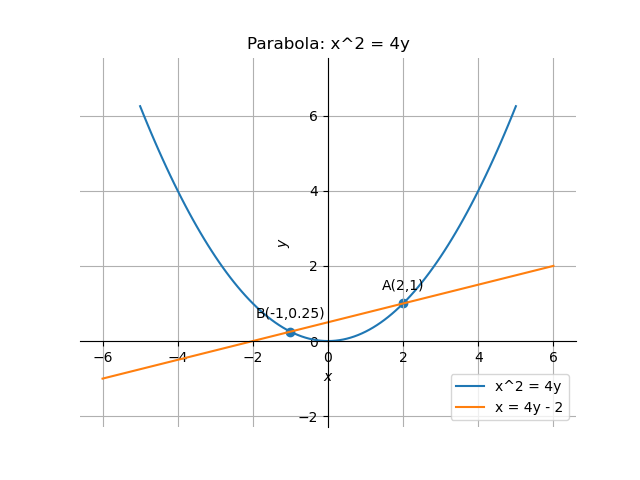
\includegraphics[scale=0.7]{figs/plot.png}
	\label{Fig}
\end{figure}
\end{document}
